% !Mode:: "TeX:UTF-8"
% 此文件从2023.11.24开始写作

\chapter{古典微分几何简介} \label{chcdg}

本章讲述三维欧几里得空间$E^3$中的一维曲线和二维曲面论;
由于高维、抽象的黎曼几何很难有具体图像,只有退化到
二维曲面才有可想象的图像,故这部分十分重要.
在这份简介中只列出主要的结论,并给出主要的证明、计算;
所忽略的定理证明、计算以及更为详尽的描述
可查阅\textcite{subq-2016}著《微分几何》.



\section{三维欧几里得空间}\label{chcdg:sec_E3}
仿射空间是与线性空间(定义见\ref{chmla:def_linear-space})相伴随的,两者既有区别又有联系.
\begin{definition}\label{chcdg:def_affine-sapce}
    设$V$是$m$维线性空间.
    $A$是一个非空集合,$A$中的元素称为{\heiti 点}.
    如果存在一个双射$\overrightarrow{\cdot \ \cdot} : A\times A \to V$,
    它把$A$中任意一对有序的点$P$、$Q$映射为$V$中的一个矢量$\overrightarrow{PQ}\in V$;
    且有$\overrightarrow{PQ}+\overrightarrow{QS}=\overrightarrow{PS}$.
    则称$A$是$m$维{\heiti 仿射空间},$V$是与$A$伴随的线性空间.
\end{definition}

\index[physwords]{仿射空间}

把定义\ref{chcdg:def_affine-sapce}中的
关系式$\overrightarrow{PQ}+\overrightarrow{QS}=\overrightarrow{PS}$三个点取成相同的点,
即$\overrightarrow{PP}+\overrightarrow{PP}=\overrightarrow{PP}$;
再由箭头“$\overrightarrow{\cdot\  \cdot}$”是双射,有$\overrightarrow{PP}=0$.

%仿射几何是一门独立的学科,可参考书籍\parencite{berger-1987}.
%在定义\ref{chcdg:def_affine-sapce}中,为了方便使用,
%我们把\parencite{berger-1987}中定义2.1.6的
%双射$\Theta(\cdot,\cdot)$换成了箭头“$\overrightarrow{\cdot\  \cdot}$”.



三维欧几里得空间$E^3$就是一个仿射空间,其伴随的线性空间是$\mathbb{R}^3$.
$\mathbb{R}^3$中的元素就是我们通常接触到的矢量(或向量),
是一个有大小、有方向的量,通常用黑体表示,比如$\boldsymbol{a}$;
常见的矢量有位移、速度、力等等.

我们在$E^3$中取定一点$O$,当作原点;然后再选取三个相互正交归一的、
固定不变的基矢量$\boldsymbol{i}$、$\boldsymbol{j}$、$\boldsymbol{k}$,它们构成右手坐标系.
由这个标架$\{O;\boldsymbol{i},\boldsymbol{j},\boldsymbol{k}\}$给出的坐标系
称为{\heiti 笛卡尔坐标系}{\footnote{        \index[persons]{笛卡尔}
Ren\'e Descartes是法国数学家,根据法语发音其名翻译为{\heiti 勒内$\cdot$笛卡尔}.
其姓氏Descartes(被认为是Des Cartes )在拉丁化后为Cartesius(译为:卡提修斯);
Cartesius发音与“笛卡尔”相去甚远.}}
或{\heiti 直角坐标系}.笛卡尔坐标系贯穿本章,不再单独声明它的存在.


设$\mathbb{R}^3$中有两个矢量$\boldsymbol{a}$、$\boldsymbol{b}$,
它们在$\{O;\boldsymbol{i},\boldsymbol{j},\boldsymbol{k}\}$上
的分量分别是$(a_1,a_2,a_3)$、$(b_1,b_2,b_3)$;
则它们的{\heiti 点乘}和{\heiti 叉乘}是(读者应非常熟悉):
\begin{align*}
    \boldsymbol{a}\cdot \boldsymbol{b} = & \bigl(a_1 \boldsymbol{i} +a_2 \boldsymbol{j}+a_3 \boldsymbol{k}\bigr) \cdot
    \bigl(b_1 \boldsymbol{i} +b_2 \boldsymbol{j}+b_3 \boldsymbol{k}\bigr)= a_1 b_1 +a_2 b_2+a_3b_3  . \\
    \boldsymbol{a}\times \boldsymbol{b} = & \bigl(a_1 \boldsymbol{i} +a_2 \boldsymbol{j}+a_3 \boldsymbol{k}\bigr) \times
    \bigl(b_1 \boldsymbol{i} +b_2 \boldsymbol{j}+b_3 \boldsymbol{k}\bigr)  \notag\\
    =&(a_1 b_2 - a_2 b_1) (\boldsymbol{i}\times \boldsymbol{j})
     +(a_2 b_3 - a_3 b_2) (\boldsymbol{j}\times \boldsymbol{k})
     +(a_3 b_1 -a _1 b_3) (\boldsymbol{k}\times \boldsymbol{i} )\\
    =& \left( \begin{vmatrix} a_2 & a_3 \\ b_2 & b_3 \end{vmatrix},\quad
    -\begin{vmatrix} a_1 & a_3 \\ b_1 & b_3 \end{vmatrix},\quad
    \begin{vmatrix} a_1 & a_2 \\ b_1 & b_2 \end{vmatrix}    \right) .
\end{align*}
设$E^3$中有两个点$A$、$B$,它们在$\{O;\boldsymbol{i},\boldsymbol{j},\boldsymbol{k}\}$上
的坐标分别是$(x_1,y_1,z_1)$、$(x_2,y_2,z_2)$;
则$\overrightarrow{AB}$的欧氏{\heiti 距离}是:
\begin{equation}
    |AB|=\sqrt{\overrightarrow{AB} \cdot \overrightarrow{AB}}
    =\sqrt{(x_2 - x_1)^2 + (y_2-y_1)^2 + (z_2-z_1)^2} .
\end{equation}



在$E^3$中再任意指定一点$P\in E^3$.
所谓$E^3$中的{\heiti 标架场}是指点$P$和其伴随矢量空间$\mathbb{R}^3$中的
一组基底$\{\boldsymbol{e}_1,\boldsymbol{e}_2,\boldsymbol{e}_3\}$组成
的总体$\{P;\boldsymbol{e}_1,\boldsymbol{e}_2,\boldsymbol{e}_3\}$;
将$E^3$中全体标架的集合记为$\widetilde{\mathscr{P}}$.
将全体正交归一标架场记为$\mathscr{P}$,显然$\mathscr{P}$是$\widetilde{\mathscr{P}}$的子集.

标架$\{P;\boldsymbol{e}_1,\boldsymbol{e}_2,\boldsymbol{e}_3\}$的基矢可能不是固定不变的,称为{\heiti 活动标架};
标架可能非正交归一,可能逐点不同;
$\{P;\boldsymbol{e}_i\}$可在$\{O;\boldsymbol{i},\boldsymbol{j},\boldsymbol{k}\}$上表示为:
\begin{equation}\label{chcdg:eqn_eAi}
\begin{cases}
    \overrightarrow{OP} = x \boldsymbol{i} + y \boldsymbol{j} + z \boldsymbol{k} , \\
    \boldsymbol{e}_1 =  a_{11} \boldsymbol{i} + a_{21} \boldsymbol{j} + a_{31} \boldsymbol{k} , \\
    \boldsymbol{e}_2 =  a_{12} \boldsymbol{i} + a_{22} \boldsymbol{j} + a_{32} \boldsymbol{k} , \\
    \boldsymbol{e}_3 =  a_{13} \boldsymbol{i} + a_{23} \boldsymbol{j} + a_{33} \boldsymbol{k} .
\end{cases}    
\end{equation}
我们要求上式中的标架是正交归一的且是右手的,即
\begin{align}
    &\boldsymbol{e}_i \cdot \boldsymbol{e}_j = \sum_{k=1}^{3} a_{ik} a_{jk} = \delta_{ij}
    =\begin{cases}  1,& i=j, \\ 0,& i\neq j. \end{cases} \quad
    1 \leqslant i,j \leqslant 3. \\
    & \boldsymbol{e}_1\times \boldsymbol{e}_2 =\boldsymbol{e}_3, \quad
    \boldsymbol{e}_2\times \boldsymbol{e}_3 =\boldsymbol{e}_1, \quad
    \boldsymbol{e}_3\times \boldsymbol{e}_1 =\boldsymbol{e}_2. \\
    &(\boldsymbol{e}_1\times \boldsymbol{e}_2)\cdot \boldsymbol{e}_3 =
    \begin{vmatrix}
        a_{11}& a_{21} & a_{31} \\ a_{12}& a_{22} & a_{32} \\a_{13}& a_{23} & a_{33}
    \end{vmatrix} = 1 .
\end{align}
式\eqref{chcdg:eqn_eAi}说明变换矩阵是正交矩阵.
常见的柱坐标系、球坐标系都是活动标架.

{\heiti 矢量函数}是指从它的定义域到$\mathbb{R}^3$的映射,也就是三个有序的实函数.
比如定义在区间$[a,b]$上的矢量函数是:
\begin{equation}
    \boldsymbol{r}(t) = \bigl(x(t), \  y(t),\  z(t)\bigr),\qquad t\in [a,b].
\end{equation}
如果$x(t),y(t),z(t)$都是$t$的连续(可微)函数,则称$\boldsymbol{r}(t)$是连续的(可微的).
再比如定义在二维矩形$[a,b]\times [c,d]$上的矢量函数是:
\begin{equation}
    \boldsymbol{r}(u,v) = \bigl(x(u,v), \  y(u,v),\  z(u,v)\bigr),
    \qquad u\in [a,b],\quad v\in [c,d].
\end{equation}
连续(可微)定义与一维的相仿.

矢量函数的导数与积分就是分量的导数与积分:
\begin{align*}
    &\frac{{\rm d} \boldsymbol{r}(t)}{{\rm d}t}= \frac{{\rm d} }{{\rm d}t}
    \bigl(x(t) \boldsymbol{i}+y(t) \boldsymbol{j}+z(t) \boldsymbol{k} \bigr)
    \xlongequal[\text{导数恒为零}]{\text{常矢量}\boldsymbol{i,j,k}}
     \frac{{\rm d} x(t)}{{\rm d}t} \boldsymbol{i}
    +\frac{{\rm d} y(t)}{{\rm d}t} \boldsymbol{j}
    +\frac{{\rm d} z(t)}{{\rm d}t} \boldsymbol{k} . \\
    &\int_{a}^{b}\boldsymbol{r}(t) {\rm d}t 
    \xlongequal[\text{可提到积分号外}]{\text{常矢量}\boldsymbol{i,j,k}} 
    \boldsymbol{i} \int_{a}^{b} x(t) {\rm d}t + \boldsymbol{j} \int_{a}^{b} y(t) {\rm d}t +
    \boldsymbol{k} \int_{a}^{b} z(t) {\rm d}t .
\end{align*}


\begin{proposition}\label{chcdg:thm_rrp=0}
    设有处处非零的可微矢量函数$\boldsymbol{r}(t)$,它的长度是常数的充分必要条件是:
    $\boldsymbol{r}'(t) \cdot \boldsymbol{r}(t)=0$.
\end{proposition}
\begin{proof}
    直接计算即可:
    \begin{align*}
        \frac{{\rm d} }{{\rm d}t} \left|\boldsymbol{r}(t)   \right|^2 = 
        \frac{{\rm d} }{{\rm d}t} \bigl(\boldsymbol{r}(t) \cdot \boldsymbol{r}(t)  \bigr)
        = 2 \boldsymbol{r}'(t) \cdot \boldsymbol{r}(t) .
    \end{align*}
    由上式即可看出$|\boldsymbol{r}(t) |^2$是常数的充要条件是$\boldsymbol{r}'(t) \cdot \boldsymbol{r}(t)=0$.
\end{proof}

\section{一维曲线}

\subsection{正则曲线}
设我们现实生活的$E^3$空间中有一个点$p$,当时间$t$变化时,$p$在$E^3$中描绘的轨迹是一条曲线.
我们命矢量函数$\boldsymbol{r}(t)=\overrightarrow{Op}$,则$\boldsymbol{r}(t)$的参数表示为
\begin{equation}
    \boldsymbol{r}(t) =\overrightarrow{Op}= x(t)\boldsymbol{i}+y(t)\boldsymbol{j}+z(t)\boldsymbol{k}
    =\bigl(x(t), \  y(t),\  z(t)\bigr),\quad t\in \mathbb{R}.
\end{equation}
我们称矢量函数$\boldsymbol{r}(t)$是$E^3$中的一条{\heiti 参数曲线}.
%假设$\boldsymbol{r}(t)$有足够高的连续可微性.


我们仅以平面上曲线来说明切矢量的概念(见图\ref{chcdg:pic_tangent}).
取定平面上直角坐标系$\{O;\boldsymbol{i},\boldsymbol{j}\}$,那么曲线可以表示
成$\boldsymbol{r}(t)=x(t)\boldsymbol{i}+y(t)\boldsymbol{j}$,将参数曲线$\boldsymbol{r}(t)$对$t$求导,有
\begin{equation}
    \frac{{\rm d}\boldsymbol{r}(t)}{{\rm d}t}=\lim_{\Delta t\to 0}
    \frac{\boldsymbol{r}(t+\Delta t)-\boldsymbol{r}(t)}{\Delta t}=
    x'(t)\boldsymbol{i} + y'(t)\boldsymbol{j} .
\end{equation}
上式的意义是:曲线上有点$\boldsymbol{r}(t+\Delta t)$和点$\boldsymbol{r}(t)$,两点连线
便是曲线的割线,当$\Delta t\to 0$时,割线趋于蓝色切线位置.
我们称参数曲线的切线方向矢量$\boldsymbol{r}'(t)$是该参数曲线的{\heiti 切矢量}.
此式及图\ref{chcdg:pic_tangent}生动地解释了:一条曲线的切线和微分(导数)是同一概念.

\begin{figure}[htb]
    \centering
    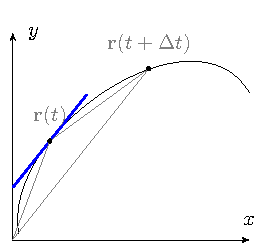
\includegraphics{fig/ch1-tangent.pdf}
    \caption{切矢量}\label{chcdg:pic_tangent}
\end{figure}


若参数曲线$\boldsymbol{r}(t)$的切矢量$\boldsymbol{r}'(t)$处处不为零,且$\boldsymbol{r}(t)$至少三次连续可微;
则称曲线$\boldsymbol{r}(t)$是{\heiti 正则曲线},并且把参数$t$增大的方向称为
曲线$\boldsymbol{r}(t)$的{\heiti 正向},故$\boldsymbol{r}'(t)$是指向正向的.

下面来处理正则曲线弧长.仍以图\ref{chcdg:pic_tangent}为例,该图中只画了
点$\boldsymbol{r}(t)$和$\boldsymbol{r}(t+\Delta t)$,先将其改记为$\boldsymbol{r}(t_i)$和$\boldsymbol{r}(t_{i+1})$,
并且设想在该曲线上存在$n+1$个这样的分点,即$a=t_0<t_1<\cdots<t_n=b$,
也就是说我给区间$[a,b]$作了一个划分(图中没有,自己想像).
当$t_i$与$t_{i+1}$无限接近时,图\ref{chcdg:pic_tangent}中的割线长度
与点$\boldsymbol{r}(t_i)$和点$\boldsymbol{r}(t_{i+1})$间的弧线长度无限接近;
这样便有(其中$\lambda = \max \{|\Delta t_i|; i=0,\cdots,n-1 \}$)
\begin{equation}\label{chcdg:eqn_arclength}
    \lim\limits_{\lambda\to 0 \atop n\to \infty } \sum_{i=0}^{n-1} 
    |\boldsymbol{r}(t_{i+1}) - \boldsymbol{r}(t_{i})| = \int_{a}^{b} |\boldsymbol{r}'(t)|{\rm d}t
    \overset{def}{=}s .
\end{equation}
上式便是曲线在$[a,b]$间的{\heiti 弧长公式};由于我们要求曲线是正则的,
故在闭区间$[a,b]$上曲线没有奇点,也不会趋于无穷远点;这样式\eqref{chcdg:eqn_arclength}中
积分一定收敛.

如果用其它参数来描述曲线,比如存在变换$t=t(u)$,则$\boldsymbol{r}(t) \to \boldsymbol{r}\bigl(t(u)\bigr)=\boldsymbol{r}(u) $;
需对变换$t=t(u)$作如下要求({\heiti 容许变换}):函数$t=t(u)$三次连续可微,并且$t'(u)>0$处处成立.
在这样要求下,这种变换并不改变曲线长度.
\begin{align*}
    s=\int_{a}^{b} |\boldsymbol{r}'(u)|{\rm d}u
     =\int_{a}^{b} \left|\frac{{\rm d}\boldsymbol{r}\bigl(t(u)\bigr)}{{\rm d}t }
     \frac{{\rm d}t(u)}{{\rm d}u}  \right|{\rm d} u
%      =\int_{a}^{b} \left|\frac{{\rm d}\boldsymbol{r}\bigl(t(u)\bigr)}{{\rm d}t }\right|
%     \frac{{\rm d}t(u)}{{\rm d}u}  {\rm d}u
     =\int_{a}^{b} |\boldsymbol{r}'(t)|{\rm d}t .
\end{align*}

现在将正则曲线$\boldsymbol{r}(u)$的弧长积分上限改为变数$t$,下限仍是固定值$a$.
\begin{align}
    s(t)=\int_{a}^{t} |\boldsymbol{r}'(u)|{\rm d}u 
    \  \xRightarrow[t \, \text{求导}]{\text{对参数}} \  
    \frac{{\rm d}s(t)}{{\rm d}t}=|\boldsymbol{r}'(t)|  > 0 .
\end{align}
上式满足{\kaishu 容许变换}要求,故总可以用弧长$s$作为正则曲线的参数.
以后为简单起见,都用弧长作为曲线的参数,称为{\heiti 自然参数};
请读者验证当选用自然参数时,有:$\boxed{|\boldsymbol{r}'(s)|=1}$.





\subsection{曲率、挠率与Frenet公式}
从上一节我们知道正则曲线$C$的切矢量$|\boldsymbol{r}'(s)|=1$;现定义:
\begin{align}
    \boldsymbol{T} (s) \overset{def}{=} \boldsymbol{r}'(s) .
\end{align}
我们研究一下这个单位长的切矢量$\boldsymbol{T} (s)$.
设正则曲线$C(s)$上有两个临近点$s$、$s+\Delta s$,此两点
的单位长切矢量分别是$\boldsymbol{T} (s)$、$\boldsymbol{T} (s+\Delta s)$.
将$\boldsymbol{T} (s+\Delta s)$平移至$s$点处,并令两个切矢量的起点重合,
它们的终点一般说来是不重合的,两者之差是$\boldsymbol{T} (s+\Delta s)-\boldsymbol{T} (s)$;
两个矢量$\boldsymbol{T} (s)$、$\boldsymbol{T} (s+\Delta s)$的夹角是$\Delta\theta$.则有
\setlength{\mathindent}{0em}
\begin{align}
    \left|\frac{{\rm d} \boldsymbol{T}}{{\rm d}s}\right| =  \lim_{\Delta s\to 0} 
    \left|\frac{\boldsymbol{T} (s+\Delta s)-\boldsymbol{T} (s)}{\Delta s}\right|
    \xlongequal{|\boldsymbol{T}|=1}
    \lim_{\Delta s\to 0} \frac{\left|2\sin\frac{\Delta\theta}{2}\right|}{|\Delta s|}
    =\lim_{\Delta s\to 0} \frac{|\Delta \theta|}{|\Delta s|}. \label{chcdg:eqn_dads}
\end{align}\setlength{\mathindent}{2em}
式\eqref{chcdg:eqn_dads}表明:在正则曲线$C(s)$上,随着弧长$s$变化,
单位长切矢量$\boldsymbol{T} (s)$对弧长的
导数$|\frac{{\rm d} \boldsymbol{T}}{{\rm d}s}|$标志着
切矢量$\boldsymbol{T} (s)$在$E^3$中转动的快慢;
它刻画了此条曲线的{\kaishu 弯曲程度}.


    设正则曲线$C(s)$的方程是$\boldsymbol{r}(s)$,$s$是弧长参数.
    令$\boxed{\kappa(s) \equiv |\tfrac{{\rm d} \boldsymbol{T}}{{\rm d}s}|=|\boldsymbol{r}''(s)|}$,
    称$\kappa(s)$是曲线$\boldsymbol{r}(s)$在$s$处的{\heiti 曲率},
    $\frac{{\rm d} \boldsymbol{T}}{{\rm d}s}$为{\heiti 曲率矢量}.

不难证明:$C(s)$是$E^3$中一条直线的充要条件是它的曲率$\kappa(s)\equiv 0$.


假设正则曲线$C(s)$的曲率$\kappa(s)\neq 0$.因$|\boldsymbol{T}(s)|=1$,
由命题\ref{chcdg:thm_rrp=0}可知:$\boldsymbol{T}(s)\cdot \boldsymbol{T}'(s)=0$,
即$\boldsymbol{T}(s) \perp \boldsymbol{T}'(s)$.故$\boldsymbol{T}'(s)$是曲线$C$的一个法矢量,且方向完全确定,
将这个方向的单位矢量记为$\boldsymbol{N}(s)$,称为正则曲线$C(s)$的{\heiti 主法矢量};
很明显,有$\boxed{\boldsymbol{T}'(s) = \kappa(s) \boldsymbol{N}(s) }$.

由曲线$C(s)$的切矢$\boldsymbol{T}$和主法矢$\boldsymbol{N}$定义{\heiti 副法矢量}:
$    \boldsymbol{B}(s) \overset{def}{=} \boldsymbol{T}(s) \times \boldsymbol{N}(s)$.

通过以上叙述,不难得到:在$\kappa(s)\neq 0$的点,正则曲线$C(s)$存在一个
右手单位标架:$\{\boldsymbol{r}(s);\  \boldsymbol{T}(s), \boldsymbol{N}(s), \boldsymbol{B}(s) \}$;
称为曲线在该点的{\bfseries \heiti Frenet标架}.
在$\kappa(s)= 0$的点,Frenet标架定义较为复杂,我们不再讨论,
请读者参阅本章末所列文献.


我们已知$\boldsymbol{B}(s)\cdot \boldsymbol{T}(s) = 0$,对此式求导得:
\begin{align}
    0= \boldsymbol{B}'(s) \cdot \boldsymbol{T}(s) + \boldsymbol{B}(s) \cdot \boldsymbol{T}'(s)
    \ \xRightarrow [\boldsymbol{B} \cdot \boldsymbol{N}=0]{\boldsymbol{T}' = \kappa \boldsymbol{N}} \ 
    \boldsymbol{B}'(s) \cdot \boldsymbol{T}(s) =0 .
\end{align}
又因$|\boldsymbol{B}(s)|=1$,故$\boldsymbol{B}(s) \cdot \boldsymbol{B}'(s)=0$;
最终,$\boldsymbol{B}'(s) \parallel \boldsymbol{N}(s)$.
不妨假设:
\begin{equation}
    \boldsymbol{B}'(s)=-\tau(s) \boldsymbol{N}(s) .
\end{equation}
上式中的$\tau(s)$为正则曲线$C(s)$的{\heiti 挠率}.
易得$\tau(s)= - \boldsymbol{B}'(s) \cdot \boldsymbol{N}(s)$和$|\tau(s)|=|\boldsymbol{B}'(s)|$.

可以证明:非直线的正则曲线$C(s)$是平面曲线的充要条件是它的挠率为零.


因$|\boldsymbol{N}(s)|=1$,故$\boldsymbol{N}(s) \cdot \boldsymbol{N}'(s)=0$;
故可设$\boldsymbol{N}'(s)=a \boldsymbol{T}(s) + c \boldsymbol{B}(s)$,则有
\begin{align*}
    a = \boldsymbol{T} \cdot \boldsymbol{N}' = -\boldsymbol{T}' \cdot \boldsymbol{N} = - \kappa(s), \quad
    c = \boldsymbol{B} \cdot \boldsymbol{N}' = -\boldsymbol{B}' \cdot \boldsymbol{N} = \tau(s). 
\end{align*}
最后,可将本小节中的公式总结为:
\begin{subequations}\label{chcdg:eqn_Frenet}
    \begin{align}
        \boldsymbol{r}'(s) =& \hphantom{-\kappa(s)} \boldsymbol{T}(s) \label{chcdg:eqn_Freneta} \\
        \boldsymbol{T}'(s) =& \hphantom{-\kappa(s) \boldsymbol{T}(s) - }
           \kappa(s) \boldsymbol{N}(s) \label{chcdg:eqn_Frenetb}\\
        \boldsymbol{N}'(s) =& -\kappa(s) \boldsymbol{T}(s) \hphantom{-\kappa(s) \boldsymbol{N}(s), }
           +\tau(s) \boldsymbol{B}(s) \label{chcdg:eqn_Frenetc}\\
        \boldsymbol{B}'(s) =& \hphantom{-\kappa(s) \boldsymbol{T}(s)} 
         -\tau(s) \boldsymbol{N}(s)  \label{chcdg:eqn_Frenetd}
    \end{align}
\end{subequations}
式\eqref{chcdg:eqn_Frenet}称为{\bfseries \heiti Frenet--Serret公式},
这是$E^3$一维曲线论中最重要的公式.

\section{二维曲面基本属性}


相对来说,$E^3$一维曲线论较为简单,而$E^3$的二维曲面论则要复杂的多;
我们将分数节来讨论这个议题.二维曲面论中的理论,经过改造后可以形式不变
地推广到高维流形上.首先给出正则曲面的定义.

我们将$E^2$中的一个连通开子集$D$映射到$E^3$中,即$S:D\to E^3$;
并在$E^2$、$E^3$中分别建立了笛卡尔坐标系,用$(u,v)$表示$E^2$中的点,
用$(x,y,z)$标记$E^3$中的点,则{\kaishu 参数曲面}$S$可以表示为:
\begin{equation}
    \boldsymbol{r}(u,v) = \bigl(x(u,v), \  y(u,v),\  z(u,v)\bigr),
    \qquad (u,v)\in D.
\end{equation}
假设$x$、$y$、$z$对$u$、$v$有三次以上的连续可微偏导数,以后不再单独声明.


设曲面$S$在$p\in S$点(坐标是$u_0,v_0$)有两个切矢量
\begin{equation}\label{chcdg:eqn_rurv}
    \boldsymbol{r}_u (u_0,v_0) \equiv \left. \frac{\partial \boldsymbol{r}}{\partial u} \right|_{(u_0,v_0)},\qquad
    \boldsymbol{r}_v (u_0,v_0) \equiv \left. \frac{\partial \boldsymbol{r}}{\partial v} \right|_{(u_0,v_0)}.
\end{equation}
若这两个切矢量是线性无关的,即$(\boldsymbol{r}_u\times   \boldsymbol{r}_v)|_{(u_0,v_0)} \neq 0$,
则称曲面$S$在$p$点{\heiti 正则};若曲面$S$上每一点都是正则的,则称之为{\heiti 正则曲面}.
之后,我们只讨论正则曲面,不再声明.


%\subsection{切平面和法矢量}

不难看出,$S$上任意一条连续可微参数曲线可以表示成:$u=u(t),\ v=v(t)$,
其中$t$是实参数;把它写成$E^3$中曲线参数方程为:
\begin{equation}
    \boldsymbol{r}= \boldsymbol{r}\bigl( u(t), v(t) \bigr),\qquad t\in \mathbb{R} .
\end{equation}

设曲面$S$有$p$点,经过$p$的任意一条曲线在该点的切矢量称为曲面$S$在$p$点的{\heiti 切矢量}.
显然,式\eqref{chcdg:eqn_rurv}中的$\boldsymbol{r}_u,\boldsymbol{r}_v$是$p$点的切矢量,
称它们为$p$点的{\heiti 自然切矢量};
其实过$p$点的任意切矢量都可以表示成自然切矢量的线性组合,即
\begin{align}
    \left. \frac{{\rm d}\boldsymbol{r}(u,v)}{{\rm d} t} \right|_{t=t_0}
    = \frac{\partial \boldsymbol{r}}{\partial u} \frac{{\rm d}u }{{\rm d} t}
     +\frac{\partial \boldsymbol{r}}{\partial v} \frac{{\rm d}v }{{\rm d} t}
     =\boldsymbol{r}_u \frac{{\rm d}u }{{\rm d} t} + \boldsymbol{r}_v \frac{{\rm d}v }{{\rm d} t}.
\end{align}
上式中切矢均在$p$点取值.
反之,如果点$p\in S$处有矢量
\begin{equation}
    \boldsymbol{v}= \alpha \boldsymbol{r}_u + \beta \boldsymbol{r}_v,\quad
    \text{切矢均在$p$点取值,常数}\alpha,\beta \in \mathbb{R} .
\end{equation}
则曲面$S$上一定存在一条过$p$点的曲线$C(t)$使得它在$p$点切矢量是$\boldsymbol{v}$.令
\begin{equation}
    u(t)=u_0 + \alpha (t-t_0),\quad v(t)=v_0 + \beta (t-t_0) ,
\end{equation}
于是$S$上曲线
\begin{equation}
    \boldsymbol{r}=\boldsymbol{r}\bigl( u(t), v(t) \bigr)
    =\boldsymbol{r}\bigl(u_0 + \alpha (t-t_0),\ v_0 + \beta (t-t_0) \bigr) .
\end{equation}
便满足这个要求;直接对上式求导就可验证.

由此可以得出:曲面$S$上过$p$点所有曲线的切矢量构成一个二维线性空间;
我们称这个二维线性空间为曲面$S$在$p$点的{\heiti 切平面},记为$T_pS$;
切平面上的矢量称为曲面$S$在$p$点的{\heiti 切矢量};
$\boldsymbol{r}_u|_{(u_0,v_0)},\boldsymbol{r}_v|_{(u_0,v_0)}$是$T_pS$的一组基矢量.

由于曲面是正则的,故$T_pS$的法矢量可按如下方式定义
\begin{equation}\label{chcdg:eqn_Snormal}
    \boldsymbol{n}(u_0,v_0) \overset{def}{=} \left. \frac{\boldsymbol{r}_u \times \boldsymbol{r}_v}
    {|\boldsymbol{r}_u \times \boldsymbol{r}_v|} \right |_ {(u_0,v_0)}
    = \frac{\boldsymbol{r}_u \times \boldsymbol{r}_v} {\sqrt{EG-F^2}}.
\end{equation}
这样,$(\boldsymbol{r}_u , \boldsymbol{r}_v, \boldsymbol{n})$构成了$p$点的$E^3$中一个右手标架;
当$p$点遍历$S$上每一点时,这个标架构成一个标架场,
称为正则曲面$S$的{\heiti 自然标架场}.
曲面$S$上任意一个矢量,不论它是否属于$S$的切平面,只要起始点在$S$上,
都可以在这个标架场下展开.



\section{第一、第二基本形式}
设正则曲面$S$上有两个两临近的点$p(u,v)$及$p'(u+\Delta u, v+\Delta v)$,
它们的矢径分别是$\boldsymbol{r}(u,v)$、$\boldsymbol{r}(u+\Delta u, v+\Delta v)$.
于是,在$E^3$中可以应用Taylor展开式,不难得到
\begin{equation*}
    \overrightarrow{pp'}=\Delta \boldsymbol{r} =\boldsymbol{r}(u+\Delta u, v+\Delta v) - \boldsymbol{r}(u,v)
    = \boldsymbol{r}_u \Delta u + \boldsymbol{r}_v \Delta v + O(\Delta u^2, \Delta v^2).
\end{equation*}
故由上式可以得到矢径的微分关系(只取线性部分)如下:
\begin{equation}\label{chcdg:eqn_drdudv}
    {\rm d} \boldsymbol{r} = \boldsymbol{r}_u {\rm d} u + \boldsymbol{r}_v {\rm d} v .
\end{equation}
当$p'$点无限接近$p$点时,也就是$\Delta u\to 0, \Delta v\to 0$,
我们就把$\overrightarrow{pp'}$在$E^3$中的长度的主部定义为曲面$S$上
这两个无限接近点的距离${\rm d}s$,即有
\begin{equation*}
    ({\rm d}s)^2 = {\rm d}\boldsymbol{r}\cdot {\rm d}\boldsymbol{r}
%    = (\boldsymbol{r}_u {\rm d} u + \boldsymbol{r}_v {\rm d} v)\cdot (\boldsymbol{r}_u {\rm d} u + \boldsymbol{r}_v {\rm d} v)
    = \boldsymbol{r}_u\cdot\boldsymbol{r}_u ({\rm d}u)^2 +2\boldsymbol{r}_u\cdot\boldsymbol{r}_v {\rm d}u {\rm d}v
    + \boldsymbol{r}_v\cdot\boldsymbol{r}_v ({\rm d}v)^2.
\end{equation*}
定义
\begin{equation}
    E\equiv \boldsymbol{r}_u\cdot\boldsymbol{r}_u, \qquad
    F\equiv \boldsymbol{r}_u\cdot\boldsymbol{r}_v, \qquad
    G\equiv \boldsymbol{r}_v\cdot\boldsymbol{r}_v .
\end{equation}
则有
\begin{equation}\label{chcdg:eqn_Iform}
    {\rm I}\equiv {\rm d}s^2 = E {\rm d}u^2 + 2 F {\rm d}u {\rm d}v + G {\rm d}v^2.
\end{equation}
这个二次微分式就是曲面$S$的{\heiti 第一基本形式},也称为曲面的{\heiti 线元};
而$E,F,G$称为曲面$S$的{\heiti 第一基本形式系数};我们已把第一基本形式记为${\rm I}$.

由于第一基本形式是个内积,即${\rm d}\boldsymbol{r}\cdot {\rm d}\boldsymbol{r}$,故它是正定二次型,即
\begin{equation}
    E>0,\quad G>0,\quad  EG -F^2 >0 .
\end{equation}

设$C(t)$是正则曲面$S$上一条正则曲线,它的参数方程为:
$\boldsymbol{r}=\boldsymbol{r}\bigl(u(t),v(t)\bigr)$,其中$a\leqslant t\leqslant b$.
从第一基本形式可以得到这条曲线的线长为
\begin{equation}
    L=\int_{a}^{b} {\rm d}s = \int_{a}^{b}
    \sqrt{E \Bigl(\frac{{\rm d}u }{{\rm d}t}\Bigr)^2 
      + 2 F \frac{{\rm d}u }{{\rm d}t} \frac{{\rm d}v }{{\rm d}t} 
      + G \Bigl(\frac{{\rm d}v }{{\rm d}t}\Bigr)^2 } \ {\rm d}t.
\end{equation}


现考虑正则曲面$S$上一块无穷小面积.曲面上由参数曲线
\begin{equation}
    u=u_0,\quad u=u_0+\Delta u;\quad v=v_0,\quad  v=v_0+\Delta v ;
    \quad \Delta u>0,\  \Delta v >0 .
\end{equation}
所围成的一小块,它的面积近似等于在点$\boldsymbol{r}(u_0,v_0)$处的切平面上
由矢量$(\Delta u) \boldsymbol{r}_u$和$(\Delta v) \boldsymbol{r}_v$所张成的平行四边形的面积,
而这个平行四边形面积是:
\setlength{\mathindent}{0em}
\begin{align*}
    &\bigl|(\Delta u) \boldsymbol{r}_u \times (\Delta v) \boldsymbol{r}_v \bigr|
    =\sqrt{(\boldsymbol{r}_u \times \boldsymbol{r}_v)\cdot (\boldsymbol{r}_u 
        \times \boldsymbol{r}_v) } \Delta u \Delta v 
    =\sqrt{\boldsymbol{r}_u \cdot \bigl( \boldsymbol{r}_v\times 
        (\boldsymbol{r}_u \times \boldsymbol{r}_v) \bigr)} \Delta u \Delta v \\
    =&\sqrt{\boldsymbol{r}_u \cdot \bigl( (\boldsymbol{r}_v\cdot\boldsymbol{r}_v)\boldsymbol{r}_u  
        -(\boldsymbol{r}_v \cdot \boldsymbol{r}_u)\boldsymbol{r}_v \bigr)} \Delta u \Delta v 
    =\sqrt{EG-F^2}    \Delta u \Delta v  .
\end{align*}\setlength{\mathindent}{2em}
此式也完成了式\eqref{chcdg:eqn_Snormal}最后一步的计算.
由上式可知曲面$S$的{\heiti 面积元素}可以表示为:
$    {\rm d}\sigma \equiv \sqrt{EG-F^2}    {\rm d} u {\rm d} v $.
曲面$S$的面积可以表示为:
\begin{equation}
    A=\iint_D {\rm d}\sigma = \iint_D \sqrt{EG-F^2}    {\rm d} u {\rm d} v .
\end{equation}



为描述曲面偏离切平面的程度,需引入第二基本形式.
在$E^3$中将$\overrightarrow{pp'}$展开到二阶:
\begin{align*}
    \overrightarrow{pp'}=&\Delta \boldsymbol{r} =\boldsymbol{r}(u+\Delta u, v+\Delta v) - \boldsymbol{r}(u,v) \\
    =& \boldsymbol{r}_u \Delta u + \boldsymbol{r}_v \Delta v + \frac{1}{2}\bigl[
    \boldsymbol{r}_{uu} (\Delta u)^2 +2\boldsymbol{r}_{uv} \Delta u \Delta v +\boldsymbol{r}_{vv} (\Delta v)^2 \bigr]
    + O(\Delta u^3, \Delta v^3).
\end{align*}
由上式可计算$p'(u+\Delta u, v+\Delta v)$点到$p(u,v)$点切平面$T_pS$的垂直距离:
\begin{equation*}
    \delta = \boldsymbol{n}\cdot \overrightarrow{pp'} = \frac{1}{2}\bigl[
    \boldsymbol{n}\cdot\boldsymbol{r}_{uu} (\Delta u)^2 +2\boldsymbol{n}\cdot\boldsymbol{r}_{uv} \Delta u \Delta v
     +\boldsymbol{n}\cdot\boldsymbol{r}_{vv} (\Delta v)^2 \bigr] + O(\Delta u^3, \Delta v^3).
\end{equation*}
Gauss引入如下记号:
\begin{equation}
    L= \boldsymbol{n}\cdot\boldsymbol{r}_{uu},\quad M= \boldsymbol{n}\cdot\boldsymbol{r}_{uv},
    \quad N=\boldsymbol{n}\cdot\boldsymbol{r}_{vv} .
\end{equation}
令$\Delta u\to 0$、$\Delta v\to 0$,则可以得到曲面$S$的{\heiti 第二基本形式}:
\begin{equation}\label{chcdg:eqn_IIform}
    {\rm II}=2\delta = L {\rm d}u^2 + 2M {\rm d}u {\rm d}v + N {\rm d}v^2 .
\end{equation}

\subsection{张量记号}
我们将第一、第二基本形式换成现代微分几何的记号,见表\ref{chcdg:tab-gauss-tensor}.

\begin{table}[htb]
    \centering
    \caption{Gauss记号和张量记号对照表} \label{chcdg:tab-gauss-tensor}
    \begin{tabular}{|*{11}{c|}}
        \hline 
        Gauss记号 & $u$   &  $v$  & $\boldsymbol{r}_u$  & $\boldsymbol{r}_v$ & $E$ & $F$ & $G$ & $L$ & $M$ & $N$ \\
        \hline
        张量记号  & $u^1$ & $u^2$ & $\boldsymbol{r}_1$ & $\boldsymbol{r}_2$ & $g_{11}$ & $g_{12},g_{21}$ & $g_{22}$ 
         & $b_{11}$ & $b_{12},b_{21}$ & $b_{22}$     \\ 
        \hline
    \end{tabular}
\end{table}

这样,二维曲面$S$的度规矩阵为
\setlength{\mathindent}{0em}
\begin{equation}\label{chcdg:eqn_2Dmetric}
    g=\begin{pmatrix} g_{11} & g_{12} \\ g_{21} & g_{22}  \end{pmatrix}
    =\begin{pmatrix} E & F \\ F & G \end{pmatrix} ; \,
    g^{-1}= \begin{pmatrix} g^{11} & g^{12} \\ g^{21} & g^{22}  \end{pmatrix}
    =\frac{1}{|g|}\begin{pmatrix} g_{22} & -g_{12} \\ -g_{21} & g_{11} \end{pmatrix} .
\end{equation}\setlength{\mathindent}{2em}
第一、第二基本形式可以表示成:
\begin{align}
    {\rm I}=& {\rm d}s^2 = g_{11} \left({\rm d}u^1\right)^2 +2g_{12} {\rm d}u^1{\rm d}u^2
      +g_{22} \left({\rm d}u^2\right)^2= \sum_{\alpha,\beta=1}^{2} g_{\alpha\beta} {\rm d}u^\alpha {\rm d}u^\beta.
       \label{chcdg:eqn_Iform-tensor} \\
    {\rm II}=& b_{11} \left({\rm d}u^1\right)^2 +2b_{12} {\rm d}u^1{\rm d}u^2
      +b_{22} \left({\rm d}u^2\right)^2= \sum_{\alpha,\beta=1}^{2} b_{\alpha\beta} {\rm d}u^\alpha {\rm d}u^\beta.
    \label{chcdg:eqn_IIform-tensor} 
\end{align}

经过数位微分几何大师的研究,终于认识到仅用$g$表示出来的二维曲面上的几何量
可以形式不变地推广到高维情形;故我们称由式\eqref{chcdg:eqn_2Dmetric}表示的
几何量为{\heiti 内蕴量},比如弧长、面积等等.
只讨论式\eqref{chcdg:eqn_2Dmetric}以及由它生成的量的几何学称为{\heiti 内蕴几何学},
由这些量决定的几何性质称为{\heiti 内蕴性质}.

涉及到第二基本形式的几何学称为{\heiti 外蕴几何学},一般说来把曲面嵌入到高维空间
的几何学都属于外蕴的.外蕴几何一般不能直接推广到高维空间.
比如类似于球面的二维曲面可以嵌入三维欧氏空间;
但像Klein瓶这种不可定向的二维流形是不能嵌入三维空间的,至少需要嵌入四维或更高维空间;
虽然都是二维流形,但被嵌入的空间以及嵌入的光滑函数必然有很大差别,
因此所涉及的外蕴几何很难以形式不变的方式推广到高维空间.




\subsection{曲面上的活动标架}
$\boldsymbol{r}_\alpha\equiv \frac{\partial \boldsymbol{r}}{\partial u^\alpha}$($\alpha=1,2$)
只是对$\boldsymbol{r}$的一次偏微分;
我们需要对它再次求偏导,即$\frac{\partial \boldsymbol{r}_\alpha}{\partial u^\beta}$;
显然$\frac{\partial \boldsymbol{r}_\alpha}{\partial u^\beta}$仍是$E^3$中的矢量,
故它可以在标架$\{\boldsymbol{r}_1,\boldsymbol{r}_2,\boldsymbol{n}\}$上展开:
\begin{equation}\label{chcdg:eqn_drdn}
    \frac{\partial \boldsymbol{r}_\alpha}{\partial u^\beta} 
    =\frac{\partial^2 \boldsymbol{r}}{\partial u^\alpha\partial u^\beta}
    = \sum_{\delta=1}^{2} \Gamma_{\alpha \beta}^\delta \boldsymbol{r}_\delta
     + c_{\alpha \beta} \boldsymbol{n};\quad
    \frac{\partial \boldsymbol{n}}{\partial u^\beta}
     = \sum_{\delta=1}^{2} \omega^\delta_\beta \boldsymbol{r}_\delta
     + c_\beta \boldsymbol{n} .
\end{equation}
我们顺带也把法矢量$\boldsymbol{n}$的微分也写了出来.下面来求出这些系数的表达式.
用单位法矢量$\boldsymbol{n}$点乘式\eqref{chcdg:eqn_drdn},
经过一些运算可得到
\begin{equation}
    c_{\alpha\beta} = b_{\alpha\beta}  \quad\text{和}\quad c_\beta=0.
\end{equation}
用$\boldsymbol{r}_\sigma$点乘式\eqref{chcdg:eqn_drdn}中第二式,
经过一些运算可得到
\begin{equation}
    \omega^\beta_\gamma = - \sum_{\sigma=1}^{2} g^{\beta \sigma} b_{\sigma\gamma}
     \overset{def}{=}b^\beta_\gamma .
\end{equation}
注意到$g_{\alpha \beta}=\boldsymbol{r}_\alpha\cdot \boldsymbol{r}_\beta$;
式\eqref{chcdg:eqn_drdn}中第一式$\boldsymbol{r}_{\alpha \beta}$、$b_{\alpha \beta}$关于
下标$\alpha$、$\beta$是对称的,
由此不难得到$\Gamma^\gamma_{\alpha \beta}=\Gamma^\gamma_{\beta\alpha}$;
用$\boldsymbol{r}_\sigma$点乘式\eqref{chcdg:eqn_drdn}中第一式,有
\begin{align}
    \boldsymbol{r}_\sigma \cdot \frac{\partial \boldsymbol{r}_\alpha}{\partial u^\beta} 
    = \sum_{\delta=1}^{2} \Gamma_{\alpha \beta}^\delta 
    \boldsymbol{r}_\delta\cdot\boldsymbol{r}_\sigma \ \Rightarrow \ 
    \frac{\partial g_{\alpha\sigma}}{\partial u^\beta} =
    \sum_{\delta=1}^{2} \left(\Gamma_{\alpha \beta}^\delta g_{\delta \sigma}
     + \Gamma_{\sigma \beta}^\delta g_{\delta \alpha} \right) . \label{chcdg:eqn_Gg}
\end{align}
轮换角标$\alpha\sigma \beta$,有
\begin{equation}
    \frac{\partial g_{\sigma\beta}}{\partial u^\alpha} =   \sum_{\delta=1}^{2} 
    \left(\Gamma_{\sigma\alpha}^\delta g_{\delta \beta} + \Gamma_{\beta\alpha}^\delta g_{\delta \sigma} \right) , \quad
    \frac{\partial g_{\beta\alpha}}{\partial u^\sigma} =   \sum_{\delta=1}^{2} 
    \left(\Gamma_{\beta \sigma}^\delta g_{\delta \alpha} + \Gamma_{\alpha \sigma}^\delta g_{\delta \beta} \right) .
\end{equation}
后两式相加再减掉第一式(注意利用$\Gamma^\gamma_{\alpha \beta}=\Gamma^\gamma_{\beta\alpha}$),得
\begin{equation}\label{chcdg:eqn_Christoffel}
    \Gamma_{\alpha\sigma}^\delta = \frac{1}{2} g^{\delta \beta}\left(\frac{\partial g_{\sigma\beta}}{\partial u^\alpha}
    +\frac{\partial g_{\beta\alpha}}{\partial u^\sigma}-\frac{\partial g_{\alpha \sigma}}{\partial u^\beta} \right) .
\end{equation}
上式说明$\Gamma_{\alpha \sigma}^\delta$只和度量有关,是内蕴量,称为{\heiti 联络系数}.
这样式\eqref{chcdg:eqn_drdn}为:
\begin{equation}\label{chcdg:eqn_GW}
    \frac{\partial \boldsymbol{r}_\alpha}{\partial u^\beta} 
    =\frac{\partial^2 \boldsymbol{r}}{\partial u^\alpha\partial u^\beta}
    = \sum_{\delta=1}^{2}\Gamma_{\alpha \beta}^\delta 
    \boldsymbol{r}_\delta + b_{\alpha \beta} \boldsymbol{n};\quad
    \frac{\partial \boldsymbol{n}}{\partial u^\beta} = 
    -\sum_{\delta=1}^{2} b_{\beta}^\delta \boldsymbol{r}_\delta .
\end{equation}
式\eqref{chcdg:eqn_GW}为二维曲面论中的{\heiti 基本公式},
第一式称为{\bfseries \heiti Gauss公式},
第二式称为{\bfseries \heiti Weingarten公式}.
这两个公式在第\ref{chsm}章有适当的推广.






\section{曲面上的曲率}
我们已对空间曲线的性质有了初步了解,定义了曲率等;
我们将借助曲线曲率来陈述曲面曲率,以及它的几何性质.
本节将会省略较多推导,请参阅\parencite[\S 2.4]{subq-2016}.

给定正则曲面$S$上的正则曲线$C(s)=\boldsymbol{r}(s)$,它的切矢量是:
$\boldsymbol{T}=\frac{{\rm d}\boldsymbol{r}}{{\rm d}s}= 
\sum_{\alpha=1}^{2}\boldsymbol{r}_\alpha \frac{{\rm d}u^\alpha}{{\rm d}s}$.
根据式\eqref{chcdg:eqn_Frenetb}可知
\setlength{\mathindent}{0em}
\begin{equation}\label{chcdg:eqn_kNn}
    \kappa \boldsymbol{N} =  \frac{{\rm d}^2\boldsymbol{r}}{{\rm d}s^2}
    = \sum_{\delta=1}^{2}\left( \frac{{\rm d}^2 u^\delta }{{\rm d}s^2} 
    + \sum_{\alpha,\beta=1}^{2}\Gamma^\delta_{\alpha\beta} 
    \frac{{\rm d}u^\alpha}{{\rm d}s}\frac{{\rm d}u^\beta}{{\rm d}s}\right) \boldsymbol{r}_\delta
    +\sum_{\alpha,\beta=1}^{2} b_{\alpha \beta}\frac{{\rm d}u^\alpha}
    {{\rm d}s}\frac{{\rm d}u^\beta}{{\rm d}s} \boldsymbol{n} .
\end{equation}\setlength{\mathindent}{2em}
由式\eqref{chcdg:eqn_kNn}可定义曲线$C(s)$的{\heiti 法曲率}$\kappa_n$:
\begin{align}
    \kappa_n \overset{def}{=} & \boldsymbol{n} \cdot (\kappa \boldsymbol{N})
    =\sum_{\alpha,\beta=1}^{2} b_{\alpha\beta}\frac{{\rm d}u^\alpha}{{\rm d}s}
    \frac{{\rm d}u^\beta}{{\rm d}s}
    =\frac{{\rm II}}{\rm I}.  \label{chcdg:eqn_kn} 
%    \kappa_g \overset{def}{=} & \sqrt{\kappa^2 -\kappa_n^2} .
\end{align}


经过略显繁琐的推导与叙述(略)可以得到:给定曲面$S$上任意一点$p$以及该点的法线$\boldsymbol{n}$;
包含法线$\boldsymbol{n}$的平面$\Pi$会在正则曲面$S$上截出一条曲线,
当$\Pi$绕着$\boldsymbol{n}$旋转一周后,所截取的曲线的法曲率会有一个最大值$\kappa_1$和
一个最小值$\kappa_2$,两者都称为{\heiti 主曲率};$\kappa_1$所对应的曲线的切矢量记为$\boldsymbol{e}_1$,
$\kappa_2$所对应的曲线的切矢量记为$\boldsymbol{e}_2$,可以证明$\boldsymbol{e}_1\cdot \boldsymbol{e}_2=0$.
由两个主曲率可以定义{\heiti 总曲率}或称为{\bfseries \heiti Gauss曲率}(高斯曲率):
\begin{equation}\label{chcdg:eqn_Gauss-Curvature}
    K \overset{def}{=}\kappa_1 \kappa_2  
    %=\det \left(\sum_{\delta=1}^{2}g^{\alpha\delta} b_{\delta\beta} \right)
    =\frac{\det b_{\alpha\beta}}{\det g_{\gamma\delta}} 
    =\frac{b_{11} b_{22} -(b_{12})^2}{g_{11} g_{22} -(g_{12})^2}
    = \frac{LN-M^2}{EG-F^2} .
\end{equation} %\setlength{\mathindent}{2em}


在$E^3$中的偏导数是可以交换次序的,比如
\begin{equation}\label{chcdg:eqn_rnuu}
    \frac{\partial^3 \boldsymbol{r}}{\partial u^\alpha \partial u^\beta \partial u^\gamma}
    =\frac{\partial^3 \boldsymbol{r}}{\partial u^\alpha \partial u^\gamma \partial u^\beta  },\qquad
    \frac{\partial^2 \boldsymbol{n}}{\partial u^\alpha \partial u^\beta }
    =\frac{\partial^2 \boldsymbol{n}}{\partial u^\beta \partial u^\alpha  } .
\end{equation}
我们将利用式\eqref{chcdg:eqn_rnuu}导出几个重要结论.
将式\eqref{chcdg:eqn_GW}带入式\eqref{chcdg:eqn_rnuu}得
\begin{align}
    \frac{\partial}{\partial u^\gamma}\left(\sum_{\delta=1}^{2}\Gamma_{\alpha \beta}^\delta \boldsymbol{r}_\delta 
    +b_{\alpha \beta}\boldsymbol{n}\right)    & =\frac{\partial}{\partial u^\beta}
    \left(\sum_{\delta=1}^{2} \Gamma_{\alpha \gamma}^\delta \boldsymbol{r}_\delta
    +b_{\alpha \gamma} \boldsymbol{n}\right), \label{chcdg:eqn_uab}  \\
    \frac{\partial}{\partial u^\gamma}\left(\sum_{\delta=1}^{2} b_\beta^\delta \boldsymbol{r}_\delta\right) 
    & =\frac{\partial}{\partial u^\beta}\left(\sum_{\delta=1}^{2} b_\gamma^\delta \boldsymbol{r}_\delta\right) . \label{chcdg:eqn_nab}
\end{align}
将式\eqref{chcdg:eqn_uab}展开,并且再次用式\eqref{chcdg:eqn_GW},整理之后得到:
\begin{align*}
    &\sum_{\delta=1}^{2}\left(\frac{\partial}{\partial u^\gamma} \Gamma_{\alpha \beta}^\delta
    -\frac{\partial}{\partial u^\beta} \Gamma_{\alpha \gamma}^\delta
    + \sum_{\eta=1}^{2}\left(\Gamma_{\alpha \beta}^\eta \Gamma_{\eta \gamma}^\delta
    -\Gamma_{\alpha \gamma}^\eta \Gamma_{\eta \beta}^\delta\right)
    -b_{\alpha \beta} b_\gamma^\delta+b_{\alpha \gamma} b_\beta^\delta\right) \boldsymbol{r}_\delta  \\
    &+\sum_{\delta=1}^{2}\left(\Gamma_{\alpha \beta}^\delta b_{\delta \gamma}-\Gamma_{\alpha \gamma}^\delta
     b_{\delta \beta}+\frac{\partial b_{\alpha \beta}}{\partial u^\gamma}
     -\frac{\partial b_{\alpha \gamma}}{\partial u^\beta}\right) \boldsymbol{n}=\boldsymbol{0} .
\end{align*}
由于$\{\boldsymbol{r}_1, \boldsymbol{r}_2, \boldsymbol{n}\}$是处处线性无关的,所以上式的系数必须为零,即有
\begin{align}
    &\frac{\partial}{\partial u^\gamma} \Gamma_{\alpha \beta}^\delta-\frac{\partial}{\partial u^\beta}
   \Gamma_{\alpha \gamma}^\delta+ \sum_{\eta=1}^{2}\left(\Gamma_{\alpha \beta}^\eta 
    \Gamma_{\eta \gamma}^\delta-\Gamma_{\alpha \gamma}^\eta \Gamma_{\eta \beta}^\delta\right)
    =b_{\alpha \beta} b_\gamma^\delta-b_{\alpha \gamma} b_\beta^\delta, \label{chcdg:eqn_Gauss} \\
    &\frac{\partial b_{\alpha \beta}}{\partial u^\gamma}-\frac{\partial b_{\alpha \gamma}}{\partial u^\beta}
    =\sum_{\delta=1}^{2}\left(\Gamma_{\alpha \gamma}^\delta b_{\delta \gamma}
    - \Gamma_{\alpha \beta}^\delta b_{\delta \beta}\right).     \label{chcdg:eqn_Codazzi}
\end{align}
式\eqref{chcdg:eqn_Gauss}、\eqref{chcdg:eqn_Codazzi}分别称为
{\bfseries\heiti Gauss方程}、{\bfseries\heiti Codazzi方程};
式中所有希腊字母取值范围是:$1,2$.
从式\eqref{chcdg:eqn_nab}出发会再次得到Codazzi方程.


容易看出式\eqref{chcdg:eqn_Gauss}的左边只是由曲面$S$的第一类基本量$g_{\alpha \beta}$(度规)
的不高于二阶的偏导数构成的量,我们把它记成
\begin{equation}\label{chcdg:eqn_Riemann}
    R_{\hphantom{\delta} \alpha \beta \gamma}^\delta \overset{def}{=}
    +\frac{\partial}{\partial u^\beta} \Gamma_{\alpha \gamma}^\delta
    -\frac{\partial}{\partial u^\gamma} \Gamma_{\alpha \beta}^\delta
    +\sum_{\eta=1}^{2}\left( \Gamma_{\alpha \gamma}^\eta \Gamma_{\eta \beta}^\delta
    -\Gamma_{\alpha \beta}^\eta \Gamma_{\eta \gamma}^\delta \right) .
\end{equation}
我们称$R_{\hphantom{\delta} \alpha \beta \gamma}^\delta$为曲面$S$的第一类基本量的{\heiti 黎曼记号},
它与第二基本型式无关;这个记号是黎曼在1854年引入的,它可以形式不变的推广到任意有限维空间.
可以证明式\eqref{chcdg:eqn_Riemann}中的记号是个张量,并且有诸多对称性,可参见\S\ref{chrg:sec_R04};
可以证明在二维曲面时,$R_{\hphantom{\delta} \alpha \beta \gamma}^\delta$实质上只有一个非零分量.

下面叙述Gauss绝妙定理;为此先把黎曼记号的上指标
降下来:$R_{\delta \alpha \beta \gamma}\equiv \sum_{\eta=1}^{2} 
g_{\delta \eta}R_{\hphantom{\delta} \alpha \beta \gamma}^\eta$.
由于只有一个非零分量,式\eqref{chcdg:eqn_Gauss}变为
\begin{equation}
    R_{1212}= b_{11} b_{22} - (b_{12})^2 .
\end{equation}
将上式两边除以$g_{11} g_{22} -(g_{12})^2$得到:
\begin{equation}\label{chcdg:eqn_RK2}
    \frac{R_{1212}}{g_{11} g_{22} -(g_{12})^2}= \frac{b_{11} b_{22} -(b_{12})^2}{g_{11} g_{22} -(g_{12})^2}
    \xlongequal{\ref{chcdg:eqn_Gauss-Curvature}} K  .
\end{equation}
虽然Gauss曲率\eqref{chcdg:eqn_Gauss-Curvature}包含第一、第二基本形式,
但由上式可知:实质上Gauss曲率只由第一基本形式构成.
这便是{\heiti \bfseries Gauss绝妙定理}(Theorema egregium):

\begin{theorem}\label{chcdg:thm_egregium}
    二维曲面的Gauss曲率只由它的第一基本形式决定.
\end{theorem}


其实一般情形下把绝妙定理叙述成:在局部等距映射下,Gauss曲率不变.
由于在本章我们没有引入等距的定义,故把它叙述成\ref{chcdg:thm_egregium}的形式.
Gauss绝妙定理推广到一般情形便是定理\ref{chrg:thm_isometry-Riemann};该处用到了等距概念.


1827年Gauss经过非常复杂的计算证明了上述定理,这是微分几何发展史上一个里程碑式的定理,
这开创了微分几何的一个新纪元——内蕴几何学.这个定理说明:
{\bfseries (1)} 无需把二维曲面嵌入$E^3$之中,我们只需研究第一基本形式(无需第二基本形式)便可研究
曲面的{\kaishu 弯曲情况}(总曲率);
{\bfseries (2)} 这种{\kaishu 内蕴}属性表明可以用单纯的二维语言来研究二维曲面,无需将其嵌入到$E^3$之中;
{\bfseries (3)} 两个曲面只要它们的高斯曲率处处相等,无论它们以何种方式嵌入$E^3$中,它们的弯曲属性都相同.
1854年黎曼(Gauss学生)发展了Gauss绝妙定理的内蕴思想.
在此之前,学者们一般把二维曲面嵌入到三维欧氏空间进行研究;
通过三维欧氏空间的度规(正定单位矩阵)诱导得到二维曲面的度规,
没有认识到二维度规是可以独立于二维曲面本身.
黎曼独辟蹊径,他将二维曲面本身看成一个独立的几何实体,而不仅仅是
三维欧氏空间的一个子集;由此他认识到二维曲面的第一基本形式(即今天的黎曼度规)是
加在二维曲面的一个附加结构,不是二维曲面(二维光滑流形)自带结构,两者可以分离.
然后,黎曼把二维曲面中成立的内蕴几何推广到任意有限维空间,
即今天的{\kaishu 黎曼几何}.

\begin{example}\label{chcdg:exm_torus}
	闭合圆环面(torus,即轮胎面)的黎曼曲率.
\end{example}

在$E^3$中,有笛卡尔直角坐标系$\{O;x,y,z\}$.
闭合圆环面的大圆圆心处于原点$O$,大圆位于$x-y$平面上,大圆半径为$R$.
一个半径为$r$的小圆沿着大圆绕$z$轴旋转,
这样旋转一周后的小圆便形成了闭合圆环面.要求$R>r>0$.
设大圆旋转半径与$x$轴夹角为$u$,小圆旋转半径与$x-y$平面夹角为$v$;
那么圆环面的参数方程为:
\begin{align*}
		x(u,v)= (R+r \cos v )\cos u , \quad
		y(u,v)= (R+r \cos v )\sin u , \quad
		z(u,v)= r \sin v .
\end{align*}
对上面三式取微分,有:
\begin{align*}
	{\rm d}x = & -(R+r \cos v) \sin u {\rm d}u - r \sin v \cos u  {\rm d} v, \\
	{\rm d}y = & (R+r \cos v) \cos u {\rm d}u - r \sin v \sin u  {\rm d} v, \\
	{\rm d}z = & r \cos v {\rm d}v .
\end{align*}
由此可以得到环面上线元:
\begin{equation*}
	{\rm d}s^2 = {\rm d}x^2+{\rm d}y^2+{\rm d}z^2 = (R+r \cos v)^2  {\rm d}u^2 + r^2   {\rm d}v^2.
\end{equation*}
容易读出环面在局部坐标$\{u,v\}$下的度量为:
\begin{equation*}
	g_{\alpha\beta}= \begin{pmatrix}(R+r \cos v)^2 &0 \\ 0& r^2\end{pmatrix}.
\end{equation*}
利用式\eqref{chcdg:eqn_Christoffel}计算可以得到非零克氏符:
\begin{equation}\label{chcdg:eqn_torus-Gamma}
	\Gamma^u_{uv}=\Gamma^u_{vu}=\frac{-r \sin v}{R+r \cos v},\qquad
	\Gamma^v_{uu}=\frac{1}{r}(R+r \cos v) \sin v.
\end{equation}
遂得非零黎曼曲率分量,以及Gauss曲率(见式\eqref{chcdg:eqn_Riemann}、\eqref{chcdg:eqn_RK2}):
\begin{equation}\label{chcdg:eqn_torus-curv}
	R_{1212}=r \cos v (R+r \cos v) ; \qquad  	K=\frac{\cos v}{r(R+r \cos v) } .
\end{equation}
式\eqref{chcdg:eqn_torus-curv}中Gauss曲率的分母必然大于零,而分子可正、可负、可零.
\qed


\begin{exercise}
	{\bfseries (1)}补全例题\ref{chcdg:exm_torus}中式\eqref{chcdg:eqn_torus-Gamma}的计算过程,包括为零的部分的计算.
	{\bfseries (2)}补全式\eqref{chcdg:eqn_torus-curv}的计算过程,只计算$R_{1212}$.
\end{exercise}

\begin{exercise}
	使用第一、第二基本形式的方法从新计算例题\ref{chcdg:exm_torus}.
\end{exercise}


\section{曲面上的平行移动}\label{chcdg:sec_pt}
在三维欧氏空间中平行移动是绝对的、熟知的:
把始点为$P$的矢量$\boldsymbol{v}$平移到始点为$P^{\prime}$的矢量$\boldsymbol{v}^{\prime}$,
{\kaishu 绝对平行移动}是指在同一笛卡尔坐标系下,$\boldsymbol{v}$ 和 $\boldsymbol{v}^{\prime}$的分量相同.


本节将讨论曲面上不同点处的切平面中的矢量的平行移动.
设$p(u)$、$ p(u+\mathrm{d} u)$是二维曲面$S$上的两个无限邻近点;可以把$S$想象为二维球面,
上述两个点分别是北极点$N$和$N$附近的一点.
为了简洁起见,记 $p(u)$ 为 $p$,$ p(u+\mathrm{d} u)$ 为 $p^*$;
又设 $T_p$、$ T_p^*$ 分别是 $p$、$ p^*$ 点的切平面;一般说来$T_p$和$ T_p^*$是不重合的.
什么时候才能说 $T_p$ 中的矢量 $\boldsymbol{v}$ 与 $T_p^*$ 中的矢量 $\boldsymbol{v}^*$ 是平行的呢?

我们要求{\kaishu 新平移定义}可以形式不变地推广到高维空间,故必然要求这种平移定义是内蕴的.
我们不能简单地用$E^3$中绝对平移方法将$\boldsymbol{v}^*$平移到$p$点后所得到的矢量$\boldsymbol{v}^{\prime *}$
称作为$\boldsymbol{v}^*$的平行矢量,因为这样做的话,移动后的矢量甚至可能不落在$T_p$中;
换句话说,按照绝对平移,平移后的矢量$\boldsymbol{v}^{\prime *}$不属于切平面$T_p$,
自然不能和$T_p$中的矢量$\boldsymbol{v}$作差或相比较(指内蕴方式作差,不是外蕴方式).
我们需另寻其它办法.

我们先用$E^3$中绝对平移方法将$\boldsymbol{v}^*$平移到$p$点,所得到的矢量是$\boldsymbol{v}^{\prime *}$,
然后在$E^3$中作差,即令${\rm d} \boldsymbol{v} = \boldsymbol{v}^{\prime *} -\boldsymbol{v}$;
利用式\eqref{chcdg:eqn_GW},只保留线性项,有
%\setlength{\mathindent}{0em}
\begin{align}
    {\rm d} \boldsymbol{v}= \mathrm{d} \sum_{\sigma=1}^{2} v^\sigma \boldsymbol{r}_\sigma 
    = \sum_{\sigma,\alpha,\beta=1}^{2} \left(\mathrm{d}   v^\sigma  
    + \Gamma_{\alpha \beta}^\sigma v^\alpha \mathrm{d} u^\beta  \right) \boldsymbol{r}_\sigma
    + \sum_{\sigma,\beta=1}^{2} v^\sigma b_{\sigma \beta}  \mathrm{d} u^\beta \boldsymbol{n} . 
    \label{chcdg:eqn_dvDn}
\end{align} %\setlength{\mathindent}{2em}
式\eqref{chcdg:eqn_dvDn}中最后一项是沿曲面$S$的法向$\boldsymbol{n}$的,倒数第二项是切于曲面$S$的,
属于切平面$T_p$.
如果我们将上式向切平面$T_p$投影,即只保留切于$T_p$的分量,消去法方向的分量,
则式\eqref{chcdg:eqn_dvDn}只剩下倒数第二项,并将其记为:
\begin{equation}\label{chcdg:eqn_Dv}
    {\rm D} \boldsymbol{v} \equiv \sum_{\sigma,\alpha,\beta=1}^{2} \left(\mathrm{d} v^\sigma  
    +  \Gamma_{\alpha \beta}^\sigma v^\alpha \mathrm{d} u^\beta  \right) \boldsymbol{r}_\sigma .
\end{equation}
式\eqref{chcdg:eqn_Dv}只有切于曲面$S$的分量,并且只包含内蕴量,不再含有第二基本形式;
称为$p\in S$点切平面$T_p$上矢量$\boldsymbol{v}$的{\heiti 协变微分}或{\heiti 绝对微分}.

设有曲面$S$上有正则曲线$C(s)$,矢量$\boldsymbol{v}$还定义在$C(s)$上,即$\boldsymbol{v}$的
起始点在$C(s)$上,但未必是$C(s)$的切线.对式\eqref{chcdg:eqn_Dv}除以${\rm d}s$,有
\begin{equation}\label{chcdg:eqn_Dvds}
    \frac{{\rm D} \boldsymbol{v}}{{\rm d}s} \equiv \sum_{\sigma,\alpha,\beta=1}^{2} 
    \left( \frac{\mathrm{d} v^\sigma } {{\rm d}s}
    +  \Gamma_{\alpha \beta}^\sigma v^\alpha 
    \frac{\mathrm{d} u^\beta}{{\rm d}s}  \right) \boldsymbol{r}_\sigma .
\end{equation}
式\eqref{chcdg:eqn_Dvds}称为矢量$\boldsymbol{v}$在曲线$C(s)$上的{\heiti 协变导数}.

\begin{theorem}\label{chcdg:thm_connection}
    设有二维曲面$S$,$S$上有曲线$C(s)$;
    $\boldsymbol{v}, \boldsymbol{w}$是上定义在$C(s)$上的切矢量场,
    $f$是定义在$C(s)$上的标量函数场,则有    
    {\bfseries (1)} ${\rm D}(\boldsymbol{v}+\boldsymbol{w})={\rm D} \boldsymbol{v}+{\rm D} \boldsymbol{w}$;$\ $    
    {\bfseries (2)} ${\rm D}(f \boldsymbol{v})=(\mathrm{d} f) \cdot \boldsymbol{v}+f {\rm D} \boldsymbol{v}$;%$\ $    
    {\bfseries (3)} $\mathrm{d}(\boldsymbol{v} \cdot \boldsymbol{w})=({\rm D} \boldsymbol{v}) 
    \cdot \boldsymbol{w} +\boldsymbol{v} \cdot {\rm D} \boldsymbol{w}$.
\end{theorem}
\begin{proof}
    (1)、(2) 是容易验证的.下面证明第(3)条.
    \begin{align*}
        & ({\rm D} \boldsymbol{v}) \cdot \boldsymbol{w} + \boldsymbol{v} \cdot {\rm D} \boldsymbol{w} \\
        &=  \sum_{\sigma,\alpha,\beta=1}^{2} \left(\mathrm{d} v^\sigma  
        +  \Gamma_{\alpha \beta}^\sigma v^\alpha \mathrm{d} u^\beta  \right) \boldsymbol{r}_\sigma 
         \cdot \boldsymbol{w} + \boldsymbol{v} \cdot 
           \sum_{\sigma,\alpha,\beta=1}^{2} \left(\mathrm{d} w^\sigma  
           +  \Gamma_{\alpha \beta}^\sigma w^\alpha \mathrm{d} u^\beta  \right) \boldsymbol{r}_\sigma \\
         &= \sum_{\sigma,\alpha,\beta,\pi=1}^{2} \left( g_{\pi \sigma} w^\pi  \mathrm{d} v^\sigma  
          +  g_{\pi \sigma} v^\pi  \mathrm{d} w^\sigma  
          +  g_{\pi \sigma} \Gamma_{\alpha \beta}^\sigma w^\pi v^\alpha \mathrm{d} u^\beta 
          +  g_{\pi \sigma} \Gamma_{\alpha \beta}^\sigma w^\alpha v^\pi \mathrm{d} u^\beta  \right)  \\  
         &\xlongequal{\ref{chcdg:eqn_Gg}}
         \sum_{\alpha,\pi=1}^{2} \left( g_{\pi \alpha} w^\pi  \mathrm{d} v^\alpha  
         +  g_{\pi \alpha} v^\alpha  \mathrm{d} w^\pi  
         +  w^\pi v^\alpha \mathrm{d} g_{\pi \alpha}   \right)  
         =\mathrm{d} (\boldsymbol{v} \cdot \boldsymbol{w}) .
    \end{align*} 
    本定理中前两条被推广成{\kaishu 联络}定义,见第\pageref{chccr:sec_affine-connection}页定义\ref{chccr:sec_affine-connection};
第三条是联络与度规相互容许的表达式,见第\pageref{chgd:eqn_connection-compatibility}页
式\eqref{chgd:eqn_connection-compatibility}.
    联络定义的推广并不是一帆风顺的;
    德国数学家Georg Friedrich Bernhard Riemann (1826-1866) 于1854年创立黎曼几何;
    德国数学家Elwin Bruno Christoffel (1829-1900) 于1869年引入克氏符,用来定义黎曼曲率,
    故也有人称此曲率为Riemann--Christoffel曲率;
    意大利数学家Gregorio Ricci-Curbastro (1853-1925)在1887-1896年间发展了绝对微分学,
    1900年他与自己的学生Tullio Levi-Civita (意大利数学家,1873-1941)完善了绝对微分学(即协变导数);
    1918年Levi-Civita才用平行移动解释协变导数,至此学者们意识到协变导数与度量可以分离,不必由度量唯一决定;
    直到1950年,法国数学家Jean-Louis Koszul(1921-2018) 给出矢量丛上的联络
    定义\ref{chfb:def_vb-conncection}(自然包含了仿射联络\ref{chccr:sec_affine-connection}),
    Koszul定义隐藏了局部坐标卡;
    同是1950年,同是法国数学家 Charles Ehresmann (1905-1979) 给出了一般纤维丛上的联络定义.
\end{proof}

我们需要抓住$E^3$中绝对平移的某些属性,把它应用到二维曲面;很明显不是所有
属性都能转移到二维曲面的.$E^3$中两个矢量的绝对平移有一个属性是:移动后两个
矢量的差恒为零,也就是矢量的普通微分恒为零.略加修改这个属性,即可推广到二维曲面;
我们给二维曲面上切矢量场的{\kaishu 平行}下个定义:

\begin{definition}\label{chcdg:def_pt}
    设有二维曲面$S$,$S$上有曲线$C(s)$;$\boldsymbol{v}$是定义在$C(s)$上的切矢量场,
    $\boldsymbol{v}$是{\heiti 平行的}是指它沿$C(s)$的协变导数恒为零(见式\eqref{chcdg:eqn_Dvds}),
    即$\left.\frac{{\rm D} \boldsymbol{v}}{{\rm d}s}\right|_{C(s)}=0$.
\end{definition}

使用协变导数代替普通微分是因为协变导数是内蕴的,而普通微分不是.
协变导数几何意义是清楚的,即先把$\boldsymbol{v}^*$绝对平移至$p$点,
然后再向$T_p$投影.

我们把这个新的平行移动定义应用到$E^3$上.因为$E^3$的度规是单位矩阵,
故它的所有联络系数$\Gamma^k_{ij}=0$,所以它的协变微分就是普通微分;
故新的平行移动定义在$E^3$中就是原来的绝对平移.




二维曲面上一个矢量$\boldsymbol{v}$沿闭合曲线$C(s)$按定义\ref{chcdg:def_pt}平行移动一周回到起点后,
一般说来不会和原来的矢量重合,会有一个夹角;
完成此计算需要用Gauss--Bonnet公式,可参考\parencite[\S 2.7.4]{subq-2016}或类似书籍.






\section{度量与空间分离}\label{chcdg:sec_sm}

在\S\ref{chcdg:sec_E3}中,我们并没有特别强调欧氏空间的度规(metric,也译为度量)是正定的单位矩阵;
如果读者没有接触过微分几何或拓扑学,那么往往意识不到这个度规的存在.
我们举例来说明度规与空间是分离的.
设空间是$\mathbb{R}^2$,先给出欧几里得度规和二维球面度规,它们的表达式分别为
\begin{equation}
    \delta=\begin{pmatrix}  
        1 &0 \\ 0& 1   
    \end{pmatrix};  \qquad
    g=\begin{pmatrix}  
        R^2 & 0 \\ 0 & R^2 \sin^2\theta  
    \end{pmatrix} .
\end{equation}
我们生活在地球表面;如果我们只关心短距离(比如几百米),
那么地球表面可以近似成一个二维平面,此时是欧氏度量$\delta$.
设有$A$、$B$两点,它们位于$x$轴上,$A$点坐标取为$(0,0)$,$B$点坐标取为$(\pi,0)$;
由此得两点间距离:
\begin{equation}
    \int_{(0,0)}^{(\pi,0)} {\left[({\rm d}x,{\rm d}y)\begin{pmatrix}  
        1 &0 \\ 0& 1   
    \end{pmatrix}
    \begin{pmatrix}  
        {\rm d}x \\ {\rm d}y   
    \end{pmatrix}\right]^{1/2}}
    =\int_{0}^{\pi} {\rm d}x =\pi.
\end{equation}
由于积分沿$x$轴,故上式中${\rm d}y\equiv 0$.
欧氏度量是单位矩阵,往往被忽略掉.
但是,如果你认为坐标本身(比如上述$x$轴上的$A$、$B$点)自带欧氏度量,
那就错了!度量和空间是分离的!

如果我们关心地球表面长距离的表述(比如南北极点间的距离),
此时就不能再近似成二维平面了,需用球面度量$g$.
二维球面的坐标是极角$\theta$和方位角$\phi$,
它们的取值范围是$(\theta,\phi)\in [0,\pi]\times[0,2\pi]\subset \mathbb{R}^2$,
很明显它们的定义域是空间$\mathbb{R}^2$的子集.
我们取北极点$N$的坐标是$(0,0)$(为简单起见已令方位角$\phi=0$),
南极点$S$坐标为$(\pi,0)$;它们之间的距离是
\begin{equation}
    \int_{(0,0)}^{(\pi,0)} \left[({\rm d}\theta ,{\rm d}\phi)\begin{pmatrix}  
        R^2 & 0 \\ 0 & R^2 \sin^2\theta  
    \end{pmatrix}
    \begin{pmatrix}  
        {\rm d}\theta  \\ {\rm d}\phi
    \end{pmatrix}\right]^{1/2}
    =\int_{0}^{\pi}R {\rm d}\theta=\pi R.
\end{equation}
由于我们求经线长度,故上式中${\rm d}\phi \equiv 0$.
上述例子表明:相同的空间$\mathbb{R}^2$,相同的坐标点$(0,0)$、$(\pi,0)$,
配上不同的度量会有不同的距离.
既然能配两个度量,自然可以配上无穷多个度量;故空间与度量是分离的,空间坐标不能自带度量.
同时,也能看到度量源于现实生活,不是凭空想象出来的.


既然空间与度量是分离的,那么由空间定义的矢量、张量等概念必须摆脱度量;
否则矢量、张量定义必然依附于某种特殊度量(比如欧式度量),没有普适性.
举个例子,很多时候我们把矢量定义成有大小、有方向的量;所谓的“大小”是指矢量的长度,
此处的长度自然是欧式度量(单位矩阵)给出的;矢量的这个定义无法推广到非欧几何.
再例如利用二维欧式度量(二维单位矩阵)定义的矢量、张量不能用于二维非欧曲面(例如二维球面);
原因很简单:{\kaishu 二维单位矩阵无法度量二维非欧曲面(例如二维球面).}
我们将在第\ref{chmla}章给出张量的一般性定义.

可能有的读者觉得没必要了解复杂的非欧几何;然而,我们生活在地球表面,
它近似是二维球面,它的Gauss曲率非零,是非欧几何;
非欧几何就在我们身边,了解与否完全取决于读者你自己.

\begin{remark}
	上面的“非欧几何”是指弯曲的二维黎曼流形,即可嵌入$E^3$中的Gauss曲率非零的二维曲面;
	更严谨描述见\S\ref{chrg:sec_local-EuclideanSpace}.
\end{remark}


\section*{小结}
本章扼要地复习了古典微分几何,并用后面黎曼几何中符号重新描述了古典微分几何中定理、公式;
微分几何大师们正是通过这种改写,才顺利地将二维曲面论中的结论推广到高维空间.
读者在了解后面黎曼几何知识时,请经常退化到本章二维曲面论,以便加深认知.


从本页起一直到\S\ref{chdm:sec_Euclidean-space}之前,度规只是若隐若现的出现,不会有实质性作用;
然后从\S\ref{chdm:sec_differentiable-manifold}直到\S\ref{chrg:sec_riemann}之前
都不会用到度规这个几何量;
之后,度规(微分几何的核心量之一)才会真正的起作用.


\printbibliography[heading=subbibliography,title=第\ref{chcdg}章参考文献]


\endinput
